
\section{Rendering Pipeline}

Die Rendering Pipeline ist eine Reihe von Aufgaben, die ausgeführt wird, um Grafik auf der GPU zu berechnen (OpenGL: \cite{gl_rendering_pipeline}; Direct3D: \cite{d3d_graphics_pipeline}). Die nachfolgenden Kapitel erklären den genauen Aufbau dieser Pipeline.

\subsection{Shader}
Ein Shader ist ein einzelnes Programm, das auf der GPU ausgeführt werden kann. Sie haben, ähnlich wie Programme, die zum Beispiel in C oder Java geschrieben sind, eine \texttt{main}-Funktion, die alle auszuführenden Befehle enthält.

Shader werden in eigenen Sprachen geschrieben, die von Grafik API zu Grafik API unterschiedlich sind. OpenGL (und Vulkan) nutzen GLSL\footnote{Eigentlich nutzt Vulkan kein GLSL, sondern ein Bytecode Format namens SPIR-V. Da dieser Bytecode allerdings nicht von Menschen geschrieben werden kann, ist im Vulkan SDK ein Cross-Compiler von GLSL zu SPIR-V enthalten, der es ermöglicht, Shader für Vulkan in GLSL zu implementieren.\cite{vk_shader}} (OpenGL Shading Language) (OpenGL: \cite{gl_shader}; Vulkan: \cite{vk_shader}) und Direct3D nutzt HLSL (High Level Shading Language) \cite{d3d_shader}. Metal nutzt ebenfalls eine eigene Sprache\cite{metal_shader}.

GLSL und HLSL sind an C angelehnte Sprachen (GLSL: \cite{gl_core_glsl}; HLSL: \cite{d3d_shader}). Die Metal Shading Language ist an C++ angelehnt (beziehungsweise baut sie auf C++14 Standard auf)\cite{metal_shader}. Alle aufgeführten Sprachen haben allerdings zusätzliche Funktionalitäten, die für die Berechnung von Grafik benötigt werden. Zudem haben sie eingebaute Bibliotheken für Mathematik (vor allem Vektor und Matrizen)(GLSL: \cite{gl_core_glsl_datatypes}; HLSL: \cite{d3d_shader_datatypes}; Metal Shading Language: \cite{metal_shader}).

\subsection{Verticies}
Ein Vertex (plural Verticies) ist ein Punkt im dreidimensionalen Raum, mit dem nutzerdefinierte Daten assoziiert werden. Üblicherweise ist mit einem Vertex mindestens eine 3D Koordinate assoziiert (dies muss allerdings nicht sein, Verticies können auch ohne eine Koordinate existieren), in der Regel aber noch viel mehr (z.B. eine sog. UV-Koordinate, die zum Texture-Mapping verwendet wird). Verticies werden genutzt, um grundlegende Flächen (sog. Primitives) zu bilden. So bilden beispielsweise drei Verticies die Eckpunkte eines Dreieckes, dessen Fläche beispielsweise mit einer Farbe oder einer Textur gefüllt werden kann. Mit Hilfe dieser Primitives lassen sich dann komplexere Formen bilden. Zwei Dreiecke führen zu einem Viereck und mit sechs Vierecken ist es möglich einen Würfel zu bauen\footnote{Es wäre auch möglich direkt ein Viereck aus vier Verticies zu bilden, es ist allerdings üblich ausschließlich Dreiecke zu nutzen und daraus komplexere Strukturen zu bauen}. Es ist ebenfalls möglich, dass ein Primitive nur eine oder zwei Verticies hat, in diesen Fällen repräsentieren sie einen Punkt beziehungsweise eine Linie.

Verticies werden auf CPU-Seite definiert und dann von der Grafik API an die Grafikkarte weiter gegeben (siehe Kapitel \ref{sec:buffer:vertexbuffer}).

\subsection{Stages}
Die Rendering Pipeline besteht aus mehreren so genannten Stages. Manche dieser Stages sind durch einen Shader programmierbar. Andere Stages sind jedoch nicht frei programmierbar, aber dennoch durch Funktionen in der Grafik API anpassbar.

Im Folgenden werden die durch Shader anpassbaren Stages ``programmierbar`` und die nicht durch Shader anpassbaren Stages ``fest definiert`` genannt.

\begin{figure}
    \caption{Die verschiedenen Shader Stages. Grau hinterlegte Stages sind programmierbar, weiß hinterlegte sind es nicht. Stages mit einem gestricheltem Rahmen sind optional. (OpenGL: \cite{gl_rendering_pipeline}; Direct3D: \cite{d3d_graphics_pipeline})}
    \label{fig:stages}
    \begin{center}
        \begin{tikzpicture}            
            \coordinate (POS_A) at (0.0,7.0);
            \coordinate (POS_B) at (0.0,6.0);
            \coordinate (POS_C) at (0.0,5.0);
            \coordinate (POS_D) at (0.0,4.0);
            \coordinate (POS_E) at (0.0,3.0);
            \coordinate (POS_F) at (0.0,2.0);
            \coordinate (POS_G) at (0.0,1.0);
            \coordinate (POS_H) at (0.0,0.0);

            \node (A) at (POS_A) [draw, minimum width=\linewidth / 2] {Vertex Specification};
            \node (B) at (POS_B) [draw, minimum width=\linewidth / 2, fill=grey] {Vertex Shader};
            \node (C) at (POS_C) [draw, minimum width=\linewidth / 2, fill=grey, dashed] {Tesselation Shader};
            \node (D) at (POS_D) [draw, minimum width=\linewidth / 2, fill=grey, dashed] {Geometry Shader};
            \node (E) at (POS_E) [draw, minimum width=\linewidth / 2] {Vertex Post-Processing};
            \node (F) at (POS_F) [draw, minimum width=\linewidth / 2] {Rasterisation};
            \node (G) at (POS_G) [draw, minimum width=\linewidth / 2, fill=grey, dashed] {Fragment Shader};
            \node (H) at (POS_H) [draw, minimum width=\linewidth / 2] {Per-Sample Operations};
            
            \draw[->] (A) edge (B);
            \draw[->] (B) edge (C);
            \draw[->] (C) edge (D);
            \draw[->] (D) edge (E);
            \draw[->] (E) edge (F);
            \draw[->] (F) edge (G);
            \draw[->] (G) edge (H);
        \end{tikzpicture}
    \end{center}
\end{figure}

Abbildung \ref{fig:stages} zeigt die verschiedenen Stages und die Reihenfolge in der diese ausgeführt werden.

\subsubsection{Vertex Specification Stage}
Die Vertex Specification Stage ist eine fest definierte Stage. Sie verarbeitet die Vertex Daten, die von der CPU an die GPU gegeben werden, und bereitet sie darauf vor, von dem Rest der Pipeline genutzt zu werden. (OpenGL: \cite{stage_gl_vertex_spec}; Direct3D: \cite{stage_d3d_vertex_spec})

\subsubsection{Vertex Shader Stage}
\paragraph{Funktionalität}
Die Vertex Shader Stage ist die erste von einem Nutzer programmierbare Stage. Der Shader wird für jeden einzelnen Vertex ausgeführt, und jeder Vertex Shader hat als Eingabedaten die Daten das jeweiligen Verticies, für das er ausgeführt wird. Es ist dann möglich, die Daten des jeweiligen Verticies zu verändern (zur Erinnerung: ``die Daten`` ist ein sehr allgemeiner Begriff, da es einem Programmierer überlassen ist, welche Daten mit einem Vertex assoziiert sind. Wenn aber beispielsweise eine 3D Koordinate mit einem Vertex assoziiert ist, dann ließe sich diese Koordinate im Vertex Shader verändern). (OpenGL: \cite{stage_gl_vertex_spec}; Direct3D: \cite{stage_d3d_vertex_shader})

\paragraph{Sinn}
Die Daten der Verticies im Shader zu verändern scheint sinnlos zu sein, schließlich könnte man dies auch auf CPU Seite machen. Allerdings wären die Möglichkeiten ohne den Vertex Shader stark eingeschränkt. Soll z.B. eine Kamera durch eine virtuelle Welt bewegt werden, ist dies nur durch die Vertex Shader Stage möglich. Das hat den Grund, dass die Kamera in Grafik APIs generell statisch ist, sie kann also nicht bewegt werden (siehe Kapitel \ref{sec:buffer:ndc}). Um dennoch eine sich bewegende Kamera zu simulieren, wird stattdessen die gesamte Welt um den Kamera herum bewegt, anstatt dass die Kamera selbst bewegt wird. Um wiederum die gesamte Welt zu bewegen, müssen die Positionen von \textit{allen} Verticies angepasst werden \footnote{In diesem Beispiel wird davon ausgegangen, dass die Verticies mindestens Positionsdaten mit sich assoziiert haben.} (und das für jedes Bild!). Dies ist eine enorme Anzahl von Berechnung, die allerdings sehr gut parallelisierbar ist. Die CPU wäre davon allerdings überfordert, da sie, wie in Kapitel \ref{sec:graphicsapis:hardware} erläutert wurde, für sehr viele, parallelisierbare Operationen im Vergleich zu einer GPU ungeeignet ist. Zudem müsste man, würde man die Vertex Positionen pro Bild auf der CPU Seite berechnen, diese ebenfalls pro Bild an die GPU schicken. Hierfür ist die Speicheranbindung von CPU zu GPU schlicht zu langsam.

\subsubsection{Tesselation Shader Stage}
(OpenGL: \cite{stage_gl_tesselation}; Direct3D: \cite{stage_d3d_tesselation})
\begin{figure}
    \newcommand{\drawtri}[3]
    {
        \draw (#1 + 0.0, #2 + 0.0) -- (#1 + #3 / 2, #2 + #3) -- (#1 + #3, #2) -- cycle;

        \fill (#1 + 0.0, #2 + 0.0) circle (1pt);
        \fill (#1 + #3 / 2, #2 + #3) circle (1pt);
        \fill (#1 + #3, #2) circle (1pt);
    }

    \caption{Ein Dreieck vor (links) und nach (rechts) der Tesselation Shader Stage ($Tesselation Level=4$).}
    \label{fig:tesselation}
    \begin{center}
        \begin{tikzpicture}
            \drawtri{0.0}{0.0}{3}
        \end{tikzpicture}
        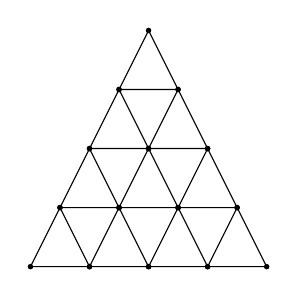
\begin{tikzpicture}
            \drawtri{0.0}{0.0}{0.75}
            \drawtri{0.75}{0.0}{0.75}
            \drawtri{1.5}{0.0}{0.75}
            \drawtri{2.25}{0.0}{0.75}

            \drawtri{0.75 / 2}{0.75}{0.75}
            \drawtri{0.75 / 2 + 0.75}{0.75}{0.75}
            \drawtri{0.75 / 2 + 1.5}{0.75}{0.75}

            \drawtri{0.75}{1.5}{0.75}
            \drawtri{1.5}{1.5}{0.75}

            \drawtri{0.75 + 0.75 / 2}{2.25}{0.75}
        \end{tikzpicture}
    \end{center}
\end{figure}

Die optionale Tesselation Stage erlaubt es, 3D Modelle mit einer geringen Anzahl an Verticies zu verfeinern, indem mehr Verticies hinzugefügt werden, bzw. indem Primitives in eine Menge kleinerer Primitives, die aber zusammen die selbe Form bilden, aufgeteilt werden. Die Anzahl der Aufteilungen bestimmt ein ganzzahliger Faktor, das sogenannte Tesselation Level. Abbildung \ref{fig:tesselation} veranschaulicht den Unterschied. 

Sehr nützlich wird die Tesselation Shader Stage dadurch, dass für jeden der hinzugefügten Verticies ein eigener Shader, der analog zu einem regulären Vertex Shader funktioniert, ausgeführt wird. Es ist also möglich, wie auch schon im Vertex Shader, die Positionen der Verticies zu verändern. Dadurch erlaubt es die Tesselation Shader Stage, einem eigentlich groberen Modell viele, deutlich feinere Details hinzuzufügen. 

Die Tesselation Shader Stage ist eine komplexe und fortgeschrittene Shader Stage. Sie besteht eigentlich aus drei unterschiedlichen Stages, die aber alle zusammen arbeiten, um das beschriebene Ergebnis zu erzielen. Diese verschiedenen Stages sind die Tesselation Control Shader Stage (programmierbar), die Tesselation Primitive Generation Stage (fest definiert) und die Tesselation Evaluatuion Shader Stage (programmierbar). 

Die Funktionsweise ist wie folgt: Tesselation geschieht auf der Basis von sogenannten Patches. Patches sind eine neue Form von Primitives, die für Tesselation verwendet werden. Sie sind Primitives, die aus einer beliebigen Anzahl von Verticies bestehen (mindestens ein Vertex und maximal 32 Verticies\footnote{Direct3D hat ein festes maximum von 32 Verticies, im Fall von OpenGL ist das maximum mindestens 32, es sind theoretisch aber auch größere Patches erlaubt. Dies wird durch die Implementierung des OpenGL Treibers bestimmt.}). Die Patches werden auf CPU Seite bestimmt. Nachdem das getan wurde, wird für jeden Patch der Tesselation Control Shader ausgeführt. Er hat als Eingabe die Vertex Daten aller Verticies im jeweiligen Patch. Seine Ausgabe pro Patch sind die (eventuell modifizierten) Vertex Daten und das Tesselation Level. Die Ausgabe Vertex Daten müssen nicht zwingend identisch zu den Eingabe Vertex Daten sein, der Shader hat also die Möglichkeit die Daten selbst zu verändern (ähnlich wie es der Vertex Shader kann) oder auch Verticies von dem Patch zu entfernen oder zu him hinzuzufügen. Das Tesselation Level bestimmt, wie oft der Patch unterteilt werden soll\footnote{In der Realität gibt es mehr als ein Tesselation Level, dies wird hier allerdings nicht weiter beachtet.}. Dadurch, dass der Tesselation Control Shader das Tesselation Level pro Patch ausgibt, ist es möglich, verschiedene Tesselation Levels innerhalb desselben Objektes zu haben. Nach dem Tesselation Control Shader wird in der Tesselation Primitive Generation Stage basierend auf der Ausgabe des Tesselation Control Shaders das Aufteilen der Patches vorgenommen. Nach diesem Schritt wird mit dem Tesselation Evaluatuion Shader der Tesselation Prozess abgeschlossen. Der Tesselation Evaluatuion Shader ist von der Funktionalität sehr nah an dem Vertex Shader, denn er wird für alle Verticies aufgerufen, die durch den vorherigen Schritt generiert worden sind und er kann für jeden dieser Verticies die Vertex Daten verändern. 

Prinzipiell wäre es auch möglich, Tesselation auf CPU Seite zu berechnen, dies würde allerdings sehr viel Rechenleistung und Bandbreite verbrauchen, da auch bei einem niedrigen Tesselation Level der Anstieg in Verticies sehr stark ist (und alle auf der CPU generierten Verticies natürlich an die GPU geschickt werden müssen). Zudem erlaubt Tesselation auf GPU Seite mehr Dynamik, da der Grad der Tesselation pro Bild verändert werden kann. Dies würde es beispielsweise erlauben, Objekten, die sehr nah an der Kamera sind, durch Tesselation mehr Details zu geben, während weiter entfernte Objekte keine Tesselation haben, um Rechenleistung zu sparen.

\subsubsection{Geometry Shader Stage}
Die Geometry Shader Stage ist erneut eine programmierbare und optionale Shader Stage. Im Gegensatz zu dem Vertex und Tesselation Shader, die auf Vertex Ebene arbeiten, arbeitet die Geometry Shader Stage auf Primitive Ebene. Sie erlaubt es, Primitives hinzuzufügen und zu entfernen. Dies kann beispielsweise genutzt werden für die Gras, ohne dass die exakten Primitives, die für deren Darstellung benötigt werden, auf CPU Seite definiert werden müssen\cite{geometry_shader_grass_prototype}. (OpenGL: \cite{stage_gl_geometry_shader}; Direct3D: \cite{stage_d3d_geometry_shader})

\subsubsection{Vertex Post Processing Stage}
\label{sec:shaderpipeline:stages:vertexpp}
\paragraph{Clipping}
Die Vertex Post Processing Stage ist hauptsächlich für das sogenannte Clipping verantwortlich. Clipping beschreibt den Vorgang, Primitives, die außerhalb des Sichtbereiches liegen, zu entfernen. Für ein Primitive bestehen dabei drei Möglichkeiten. (OpenGL: \cite{stage_gl_vertex_pp}; Direct3D: \cite{stage_d3d_vertex_pp})

\begin{figure}
    \caption{Ein Dreieck, das außerhalb des Sichtbereiches liegt, vor (links) und nach (rechts) dem Clipping. Der Sichtbereich wird durch das Viereck markiert. Hierbei wurde ein neues Primitive erzeugt (es ist allerdings nicht garantiert, dass eine reelle Grafik API sich genau so verhalten würde).}
    \label{fig:clipping}
    \begin{center}
        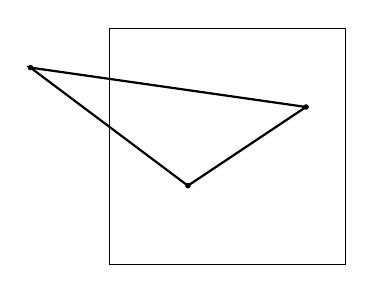
\begin{tikzpicture}
            \draw [thick] (1.0,1.0) -- (-1.0,2.5) -- (2.5,2.0)  -- cycle;

            \fill (1.0,1.0) circle (1pt);
            \fill (-1.0,2.5) circle (1pt);
            \fill (2.5,2.0) circle (1pt);

            \draw (0.0,0.0) rectangle (3.0,3.0);
        \end{tikzpicture}
        \hspace{1cm}
        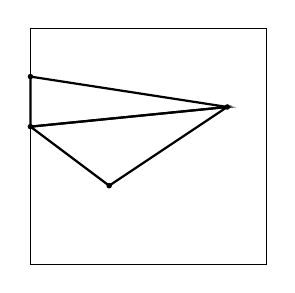
\begin{tikzpicture}
            \draw [thick] (0.0,3.5/2) -- (0.0,2+1.35/3.5) -- (2.5,2.0) -- cycle;
            \draw [thick] (1.0,1.0) -- (0.0,3.5/2) -- (2.5,2.0) -- cycle;

            \fill (1.0,1.0) circle (1pt);
            \fill (0.0,2+1.35/3.5) circle (1pt);
            \fill (0.0,3.5/2) circle (1pt);
            \fill (2.5,2.0) circle (1pt);

            \draw (0.0,0.0) rectangle (3.0,3.0);
        \end{tikzpicture}
    \end{center}
\end{figure}

\begin{enumerate}
    \item Das Primitive liegt komplett im Sichtbereich. In diesem Fall wird es nicht verändert.
    \item Das Primitive liegt komplett außerhalb des Sichtbereiches. In diesem Fall wird es komplett entfernt.
    \item Das Primitive liegt nur teilweise im Sichtbereich. In diesem Fall wird, durch das verschieben von existierenden Verticies oder das einfügen neuer Verticies, so verändert, dass das resultierende Primitive komplett im Sichtbereich liegt. Es kann sogar vorkommen, dass, wenn nötig, neue Primitives eingefügt werden. Abbildung \ref{fig:clipping} visualisiert diesen Vorgang.
\end{enumerate}

\paragraph{Depth Clamping}
Depth Clamping ist eine spezielle Version des Clippings, das sich auf die Z-Achse bezieht. Wenn Depth Clamping aktiviert ist, dann wird der übliche Wertebereich für die Z-Achse ($[-1,0;1,0]$) ignoriert und es wird stattdessen ein von einem Programmiere gesetzter Wert für das Clipping genutzt. Die X und Y Achsen bleiben durch Depth Clamping unbeeinflusst. Wenn Depth Clamping nicht aktiviert ist, gilt selbstverständlich auch für die Z Achse das übliche Interval $[-1,0;1,0]$. (OpenGL: \cite{stage_gl_vertex_pp}; Direct3D: \cite{stage_d3d_vertex_pp})

\paragraph{Direct3D Besonderheit}
Bei Direct3D ist der Vertex Post Processing Stage keine eigene Stage, sondern sie ist in der Rasterisation Stage mitinbegriffen. Dies macht für einen Programmierer allerdings keinen besonderen Unterschied, da beide Stages ohnehin fest definiert sind und sie direkt aufeinander folgen.

\subsubsection{Rasterisation Stage}
\paragraph{Funtkionalität}
Die Rasterisation Stage ist eine fest definierte Shader Stage. Sie berechnet, welche Primitives welche Pixel auf dem Ausgabemedium (z.B. Bildschirm oder Bilddatei) einnehmen. (OpenGL: \cite{stage_gl_rasterization}; Direct3D: \cite{stage_d3d_rasterization})

\paragraph{Beispiel}

\begin{figure}
    \caption{Ein Dreieck auf einem Pixel-Raster.}
    \label{fig:rasterizergfxnotfilled}
    \drawrasterizergfxnotfilled
\end{figure}

\begin{figure}
    \caption{Das selbe Dreieck wie in Abbildung \ref{fig:rasterizergfxnotfilled}, aber mit den dazugehörigen Pixeln grau eingefärbt.}
    \label{fig:rasterizergfxfilled}
    \drawrasterizergfxfilled
\end{figure}

Soll zum Beispiel das Dreieck in Abbildung \ref{fig:rasterizergfxnotfilled} gezeichnet werden, kann das nicht einfach so geschehen, sondern es muss erst bestimmt werden, welche Pixel zu dem Dreieck gehören und welche nicht. Theoretisch könnte das Ergebnis aussehen wie in Abbildung \ref{fig:rasterizergfxfilled}\footnote{Die Abbildung ist lediglich zu Visualisierungszwecken und stellt nicht unbedingt das Ergebnis einer Grafik API dar.}.

Durch Rasterisation (bzw. durch die Nutzug von Pixeln) sind die tatsächlich gezeichneten Formen nur Annäherungen an die eigentlichen Primitives. Dieses Problem ist allerdings bei einer ausreichend hohen Auflösung vernachlässigbar (die Auflösung in den Abbildungen \ref{fig:rasterizergfxnotfilled} und \ref{fig:rasterizergfxfilled} ist mit $8*8$ Pixeln sehr gering).

\subsubsection{Fragment Shader Stage}
\paragraph{Funktionalität}
(OpenGL: \cite{stage_gl_fragment_shader}; Direct3D: \cite{stage_d3d_fragment_shader})
Die Fragment Shader Stage ist erneut programmierbar und sie bestimmt hauptsächlich die Farbe und den Tiefe-Wert eines Pixels (genauer gesagt eines Fragments, siehe Paragraph \ref{sec:shaderpipeline:stages:fragshader:fragmentvspixel}). Diese Shader Stage ist optional.

Der Tiefe-Wert des Fragments wird genutzt, um zu bestimmen wie tief das jeweilige Fragment im 3D Raum liegt. Üblicherweise liegen die Fragments auf der Oberfläche, durch die sie erzeugt wurden (wenn beispielsweise ein Fragment durch ein Dreieck erzeugt wurde, liegt es genau auf dem Dreieck). Es ist dem Fragment Shader allerdings erlaubt, den Tiefe-Wert des Fragments zu verändern.

\paragraph{Sinn}
Dadurch, dass mit Hilfe der Fragment Shader Stage die Farbe von einzelnen Fragments bestimmt werden kann, ermöglicht er unter anderem per Pixel Beleuchtung\footnote{Es existiert ebenfalls per Vertex Beleuchtung, dies sieht allerdings sehr unrealistisch aus und wird in der Regel nur aus Performance Gründen genutzt} und Texture Mapping.

\paragraph{Unterschied zwischen Fragments und Pixeln}
\label{sec:shaderpipeline:stages:fragshader:fragmentvspixel}
Ein Fragment ist ein potentieller Pixel. Während ein Pixel ein tatsächlicher Bildpunkt ist, der genau eine Farbe ohne Transparent hat, kann es pro Pixel mehrere Fragmente mit verschiedenen Farben und Transparenz (aber immer nur eine Farbe pro Fragment) geben. Diese einzelnen Fragmente werden dann später zusammen verrechnet, um die endgültige Farbe des Pixels zu bestimmen. Wenn zum Beispiel eine grüne Wand hinter einer rot eingefärbten Glasscheibe steht, dann würde die Fragment Shader Stage für die Wand ein Fragment mit der Farbe grün und ohne Transparenz ausgeben und für die Glasscheibe ein Fragment mit der Farbe rot und $50\%$ Transparenz. Wenn diese beiden Fragmente von einer späteren Shader Stage zusammen gerechnet werden, dann hätte der finale Pixel die Farbe gelb (und keine Transparenz). Es ist allerdings auch möglich, dass ein Fragment direkt zu einem Pixel wird, zum Beispiel, wenn im vorherigen Beispiel die rote Glasscheibe fehlen würde oder die Wand vor der Glasscheibe ist (da die Scheibe nicht hinter der Wand sichtbar ist).

Zudem heißt die Fragment Shader Stage bei Direct3D Pixel Shader Stage. Sie berechnet dennoch Fragments und keine Pixel. Lediglich der Name ist eventuell suboptimal gewählt.

\subsubsection{Per-Sample Operations}
(OpenGL: \cite{stage_gl_per_sample_ops}; Direct3D: \cite{stage_d3d_per_sample_ops})
Die Per-Sample Operations ist die letzte Shader Stage in der Pipeline. Sie ist dafür verantwortlich, die finalen Pixel zu berechnen. In dieser Shader Stage werden viele Operationen ausgeführt, die Wichtigsten sind allerdings der Depth Test und das Color Blending.

\paragraph{Depth Test}
Wenn mehrere Fragments auf dem selben Pixel hintereinander liegen (sie sich also gegenseitig verdecken), dann bestimmt der Depth Test welches der Fragments am nähesten zur Kamera liegt (dies geschieht anhand des Tiefe-Wertes der durch den Fragment Shader berechnet wurde). Dieses Fragment wird dann zum letztendlichen Pixel und die restlichen, verdeckten Fragments, werden nicht weiter beachtet.

\paragraph{Color Blending}
Wenn mehrere Fragments auf dem selben Pixel hintereinander liegen, der vordere (bzw. die vorderen) Pixel aber einen Alpha Wert $< 100\%$ hat, dann muss die Grafik API die Fragments zusammen rechnen, sodass der resultierende Pixel die korrekte Farbe hat. Für ein Beispiel, siehe das Beispiel in Paragraph \ref{sec:shaderpipeline:stages:fragshader:fragmentvspixel}.
